\documentclass{beamer}
\setbeamertemplate{itemize items}[ball]

\usepackage{listings}
\usepackage{xcolor}
\usepackage{multicol}
\usepackage{amsmath}
\usepackage{subcaption}

\definecolor{codegreen}{rgb}{0,0.6,0}
\definecolor{codegray}{rgb}{0.5,0.5,0.5}
\definecolor{codepurple}{rgb}{0.58,0,0.82}
\definecolor{backcolour}{rgb}{0.95,0.95,0.92}

\lstdefinestyle{mystyle}{
    %backgroundcolor=\color{backcolour}, 
    commentstyle=\color{codegreen},
    keywordstyle=\color{magenta},
    numberstyle=\tiny\color{codegray},
    stringstyle=\color{codepurple},
    basicstyle=\ttfamily\footnotesize,
    breakatwhitespace=false,         
    breaklines=true,                 
    captionpos=b,                    
    keepspaces=true,                 
    numbers=left,                    
    numbersep=5pt,               
    showspaces=false,
    showstringspaces=false,
    showtabs=false,                  
    tabsize=2
}

\lstset{style=mystyle}

\usepackage{hyperref}
\hypersetup{
    colorlinks=true,
    linkcolor=blue,
    filecolor=magenta,      
    urlcolor=cyan
}

\urlstyle{same}

\title{4: Dynamic Programming - Basic Ideas}
\author{CPCFI}
\institute{UNAM's School of Engineering}
\date{2021 \\ \vspace{0.5cm} \scriptsize{Based on: Halim S., Halim F.\textit{Competitive Programming 3}}. Handbook for ACM ICPC and IOI Contestants. 2013}

\begin{document}

\frame{\titlepage}

\AtBeginSection[]
{
  \begin{frame}
    \frametitle{Table of Contents}
    \tableofcontents[
    	currentsection,
    	currentsubsection
	]
  \end{frame}
}

%-------------------------------------------------------------------------------------
%-------------------------------------------------------------------------------------
%-------------------------------------------------------------------------------------
\section{3.5 Dynamic Programming}

\subsection{0. Background}

\begin{frame}[fragile]
\frametitle{Dynamic Programming - Background}

\begin{quote}
    The most challenging algorithmic problems involve optimization, where we seek to find a solution that maximizes or minimizes and objective function
\end{quote}

\end{frame}

\begin{frame}[fragile]
\frametitle{Dynamic Programming - Background}

Algorithms for optimization problems require proof that they always return the best possible solution. 

\begin{itemize}
    \item Greedy algorithms that make best local decisions at each step are efficient but do not guarantee global optimality
    \pause
    \item Complete Search algorithms always produce the optimal solution but suffer from great time complexity
\end{itemize}

\pause
\vspace{0.3cm}

    Dynamic Programming gives us a way to design custom algorithms that \textbf{systematically search} all possibilities (guaranteeing correctness) while \textbf{storing} intermediate results to avoid recomputing (efficiency)

\end{frame}

\begin{frame}[fragile]
\frametitle{Dynamic Programming - Background}

\begin{itemize}
    \item Dynamic Programming is the fourth paradigm of algorithm construction (CS, Greedy, D\&Q) occupied for efficiently implementing a recursive algorithm by sorting partial results. 
    
    \pause
    \item It requires searching for a recursive structure that computes the same sub-problems repeatedly. Once we identify this structure, the idea is to store the answer for each sub-problem in a table to further look up the answer instead of computing again the same sub-problem.
\end{itemize}

\end{frame}

\begin{frame}[fragile]
\frametitle{Prerequisites for DP}

\begin{enumerate}
    \item The problem has optimal sub-structures
	\item The problem has overlapping sub-problems
\end{enumerate}

\vspace{1cm}

\begin{itemize}
    \item In the next subsection (\color{blue} 3.5.1 Illustration - DP Approach\color{black}), we'll see an example (UVa - 11450) where we look into detail the definition of this two prerequisites
\end{itemize}

\end{frame}

\begin{frame}[fragile]
\frametitle{How to identify a DP problem?}

\begin{itemize}
    \item DP is primarily used to solve \textit{optimization} problems and \textit{counting} problems
    \item Most DP problems will begin with "minimize this", "maximize that" or "count the ways to do that"
\end{itemize}
\end{frame}

%-------------------------------------------------------------------------------------
%-------------------------------------------------------------------------------------
%-------------------------------------------------------------------------------------
\subsection{1. Illustration}

\begin{frame}
	\frametitle{Table of Contents}
    \tableofcontents[
    	currentsection,
    	currentsubsection
	]	
\end{frame}

\begin{frame}[fragile]
\frametitle{UVa 11450 - Wedding Shopping}

\color{red}\textbf{Problem Description} \color{black} - \href{https://onlinejudge.org/external/114/11450.pdf}{UVa 11450} \\

\vspace{0.2cm}

Given different options for each garment (e.g. 3 shirt models, 2 belt models, 4 shoe models, $\ldots$ ) and a certain limited budget, our task is to buy one model of each garment. We cannot spend more money than the given budget, but we want to spend the maximum possible amount. \\

\end{frame}

\begin{frame}[fragile]
\frametitle{UVa 11450 - Wedding Shopping}

\color{red}\textbf{Input:}\color{black}

\begin{itemize}
    \item Budget $M$: $1\leq M \leq 200$
    \item Number of garments $C$: $1\leq C \leq 20$
    \item For each garment $g_i$: $g_i \in [0,\ldots,C-1]$:
    	\begin{itemize}
		    \item Number of models $K$: $1\leq K \leq 20$
		    \item Price for each model $p_i$: $p_i \in [1,\ldots,K]$
		\end{itemize} 
\end{itemize}

\vspace{0.3cm}

\color{red}\textbf{Output: }\color{black} one integer that indicates the maximum amount of money we can spend purchasing one of each garment without exceeding the budget. It is possible that there is no solution to some test cases.

\end{frame}


\begin{frame}[fragile]
\frametitle{UVa 11450 - Wedding Shopping}

\color{red}Test case $A$: \color{black} $M=20$ and $C=3$:
\begin{itemize}
    \item $K_0=3 \rightarrow \{6,4,8\}$
    \item $K_1=2 \rightarrow \{5,10\}$
    \item $K_2=4 \rightarrow \{1,5,3,5\}$        
\end{itemize}

\pause

\vspace{0.3cm}

\color{red}Solution: \color{black} \\

The answer is $19$ which may be formed with the following combinations of garments' purchases:
\begin{enumerate}
    \item $8+10+1$
    \item $6+10+3$
    \item $4+10+5$
\end{enumerate}

\end{frame}

\begin{frame}[fragile]
\frametitle{UVa 11450 - Wedding Shopping}

\color{red}Test case $B$: \color{black} $M=9$ and $C=3$:
\begin{itemize}
    \item $K_0=3 \rightarrow \{6,4,8\}$
    \item $K_1=2 \rightarrow \{5,10\}$
    \item $K_2=4 \rightarrow \{1,5,3,5\}$        
\end{itemize}

\pause

\vspace{0.3cm}

\color{red}Solution: \color{black} \\

The answer is \textit{no solution}

\end{frame}

\begin{frame}[fragile]
\frametitle{UVa 11450 - Wedding Shopping}

Now, let's explore some approaches to solve this problem...

\vspace{0.3cm}

\begin{enumerate}
    \item Greedy - \textbf{WA} verdict
    \item Complete Search - \textbf{TLE} verdict
    \item Divide and Conquer - \textbf{Not possible}
    \item Top-Down DP - \textbf{AC} verdict
    \item Bottom-Up DP - \textbf{AC} verdict
\end{enumerate}

\end{frame}

\begin{frame}[fragile]
\frametitle{UVa 11450: Greedy Approach}

Since we want to maximize the budget spent, one greedy idea (there are other greedy approaches—which also produces \textit{WA} verdict) is to take the most expensive model for each garment $g_i$ which still fits our budget. \\

\vspace{0.3cm}

This greedy idea works for test cases $A$ and $B$ and both produce the optimal solution, however, if we look into test case $C$, this strategy won't work.

\end{frame}

\begin{frame}[fragile]
\frametitle{UVa 11450: Greedy Approach}

\color{red}Test case $C$: \color{black} $M=12, C=3$:
\begin{itemize}
    \item $K_0=3 \rightarrow \{6,4,8\}$
    \item $K_1=2 \rightarrow \{5,10\}$
    \item $K_2=4 \rightarrow \{1,5,3,5\}$        
\end{itemize}

\pause
\vspace{0.3cm}

\color{red}Solution: \color{black} the greedy strategy will select for $K_0$ price $8$, for $K_1$ price $10$ and for $K_2$ price $5$ which results in a total price of $23 >> M$. Therefore, producing a \textit{no solution} answer which is incorrect.

\end{frame}

\begin{frame}[fragile]
\frametitle{UVa 11450: Complete Search Approach}

\begin{itemize}
    \item Let's start with a function \verb|shop(money, g)| where the pair \verb|(money, g)| is a state of the problem
    \pause
    \item We start with \verb|money=M| and \verb|g=0|
    \pause
    \item We try all possible models in garment $g=0$ and if model $i$ is chosen, we subtract model $i$'s price from \verb|money|
    \pause    
    \item We repeat this process recursively and stop in either the last garment or when \verb|money < 0| before reaching the last garment model
    \pause
    \item \color{blue}Among all valid combinations, we can then pick the one that results in the smallest non-negative \verb|money|\color{black}
\end{itemize}

\end{frame}

\begin{frame}[fragile]
\frametitle{UVa 11450: Complete Search Approach}

We can define the recurrences formally as follows:
\begin{enumerate}
    \item If \verb|money < 0|: 
	    \begin{itemize}
        	\item \verb|shop(money, g) = |$-\infty$
    	\end{itemize}
	\pause
    \item If a model from the last garment has been bought, i.e. $g=C$:
	    \begin{itemize}
    	    \item \verb|shop(money, g)= M - money|
	    \end{itemize}
	\pause	    
	\item $\forall$ garment model $g_i \in [1,\ldots,K]$:
		\begin{itemize}
		    \item \verb|shop(money,g)=max(shop(money-price[g][model],g+1))|
		\end{itemize}
\end{enumerate}

\end{frame}

\begin{frame}[fragile]
\frametitle{UVa 11450: Complete Search Approach}

\begin{itemize}
    \item This solution works correctly but it's \textbf{very slow}
    \item In the largest test case, garment $g = 0$ has up to $20$ models, garment $g = 1$ also has up to $20$ models and all garments including the last garment $g = 19$ also have up to $20$ models
    \item Therefore, this Complete Search solution runs in $20\times 20\times \ldots \times 20$ operations, i.e. $20^{20} = 1.04\times 10^{26}$ which produces a \textbf{Time Limit Exceeded TLE} verdict
\end{itemize}
\end{frame}


\begin{frame}[fragile]
\frametitle{UVa 11450: Divide and Conquer Approach}

\begin{itemize}
    \item This problem is not solvable using the Divide and Conquer paradigm, since the sub-problems are not independent
    \item The sub-problems are the problem's states described above in the \color{blue}Complete Search approach\color{black}
\end{itemize}
\end{frame}

\begin{frame}[fragile]
\frametitle{UVa 11450: Top-Down DP Approach}

UVa 11450 satisfies the two prerequisites for DP to be applicable:

\begin{enumerate}
    \item \color{blue}Optimal sub-structures\color{black}
	
	\begin{itemize}
	    \item The solution for the sub-problem is part of the solution of the original problem
	    \item If we select model $i$ for garment $g = 0$, for our final selection to be optimal, our choice for garments $g = 1$ and above must also be the optimal choice for a reduced budget of \verb|M - price|, where \verb|price| refers to the price of model $i$
	\end{itemize}
	
	\pause
    \item \color{blue}Overlapping sub-problems\color{black}
    	\begin{itemize}
		    \item This is the key characteristic of DP
		    \item The search space of this problem is not as big as the rough $20^{20}$ bound obtained earlier because \textbf{many} sub-problems are overlapping
		\end{itemize}
\end{enumerate}

\end{frame}

\begin{frame}[fragile]
\frametitle{UVa 11450: Top-Down DP Approach}

Are there any \textbf{repeated} (overlapping) sub-problems? 

\pause
\vspace{0.3cm}
This happens if some combination of \verb|money| and chosen model’s price causes \verb|money1 - p1 = money2 - p2| for the same garment $g$.

\end{frame}

\begin{frame}[fragile]
\frametitle{UVa 11450: Top-Down DP Approach}

So, how many distinct sub-problems are there? Considering that \verb|money| $\in [0,\ldots,200]$ and the number of garments $\in [0,\ldots,19]$.

\pause 
\vspace{0.3cm}

$$201 \times 20 = 4020 \; \text{states}$$

\pause
\vspace{0.3cm}

\color{blue}Each sub-problem must be computed only once and by ensuring this, we could solve the problem much faster.\color{black}

\end{frame}

\begin{frame}[fragile]
\frametitle{UVa 11450: Top-Down DP Approach}

In order to implement the Top-Down DP solution we must add the following steps:

\begin{enumerate}
    \item \color{blue}Initialize a DP table with dummy values that are not used in the problem\color{black}
    
    \begin{itemize}
        \item This table must have dimensions accordingly to the problem states
    \end{itemize}
    
    \pause
    \item \color{blue}At the start of the recursive function, check if this state has been computed before\color{black}
    	\begin{itemize}
		    \item If it has, return the value from the DP table $O(1)$
		    \item If it has not, perform the computation and then store the computed value in the DP table
		\end{itemize}
\end{enumerate}

\end{frame}

\begin{frame}[fragile]
\frametitle{UVa 11450: Top-Down DP Approach}

\textbf{DP analysis: }
\begin{itemize}
    \item If the problem has $M$ states, then the program will require $O(M)$ memory space
    \item If computing one state requires $O(k)$ steps, the the overall time complexity is $O(kM)$
    \item \color{red}UVa 11450 \color{black} has $M=4020$ states and $k=20$ (at most $20$ models for each garment $g$)
    \item Therefore, $80,400$ operations per test case\footnote{Recall that modern computers can perform $10^8 = 100M$ operations per second} which is ideal
\end{itemize}

\vspace{0.3cm}

\color{red}* \verb|C++ code: ch3_02_UVa11450_td.cpp| \color{black}

\end{frame}


\begin{frame}[fragile]
\frametitle{UVa 11450: Bottom-Up DP Approach}

Steps to build a bottom-up DP solution:

\begin{enumerate}
    \item Determine the required set of parameters that uniquely describe the problem (state)
	\pause
	\item If there are $N$ parameters required to represent the states, prepare an $N$ dimensional DP table, with one entry per state
		\begin{itemize}
		    \item In Bottom-Up DP, we only need to initialize some cells of the DP table with known initial values (the base cases)
		    \item In Top-Down DP, we initialize the memo table completely with dummy values (usually -1) to indicate that we have not yet computed the values
		\end{itemize}
	\pause
	\item Determine the cells/states that can be filled next (the transitions)
	\item Repeat (iterate) until the DP table is complete
\end{enumerate}

\end{frame}

\begin{frame}[fragile]
\frametitle{UVa 11450: Bottom-Up DP Approach}

Bottom-Up DP for UVa 11450: 
\begin{enumerate}
    \item Parameters: current garment $g$ and current \verb|money|
    \item Initialize a 2D boolean matrix (DP table): \color{blue}\verb|reachable[g][money]| \color{black} of size $20\times 201$
    \item Cells/states when $g=0$ are marked as true (using test case $A$'s parameters: $M=20, C=3$)
    	\begin{itemize}
		    \item \verb|reachable[0][M - 6] = 1|
		    \item \verb|reachable[0][M - 4] = 1|
		    \item \verb|reachable[0][M - 8] = 1|		    		    
		\end{itemize}
\end{enumerate}

\pause

\begin{figure}
    \centering
    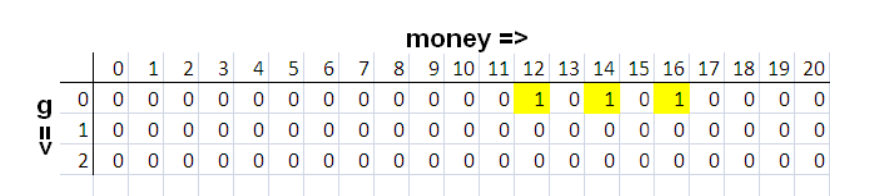
\includegraphics[scale=0.4]{imgs/11450_1.png}
    \caption{DP table for $g=0$}
\end{figure}


\end{frame}

\begin{frame}[fragile]
\frametitle{UVa 11450: Bottom-Up DP Approach}

\begin{enumerate}
	\setcounter{enumi}{3}
    \item Iterate with the remaining garments ($g=\{1,2\}$) as follows:
    	\begin{itemize}
		    \item If \verb|reachable[g-1][money]| is true, then \verb|reachable[g][money - p]| will be set to true as long as \verb|money| is not negative\footnote{$p$ is the price for garment $g_i$}
		    \item For example, \verb|reachable[0][16]| propagates to \verb|reachable[1][16-5]| and \verb|reachable[1][16-10]|
		\end{itemize}
\end{enumerate}

\begin{figure}
    \centering
    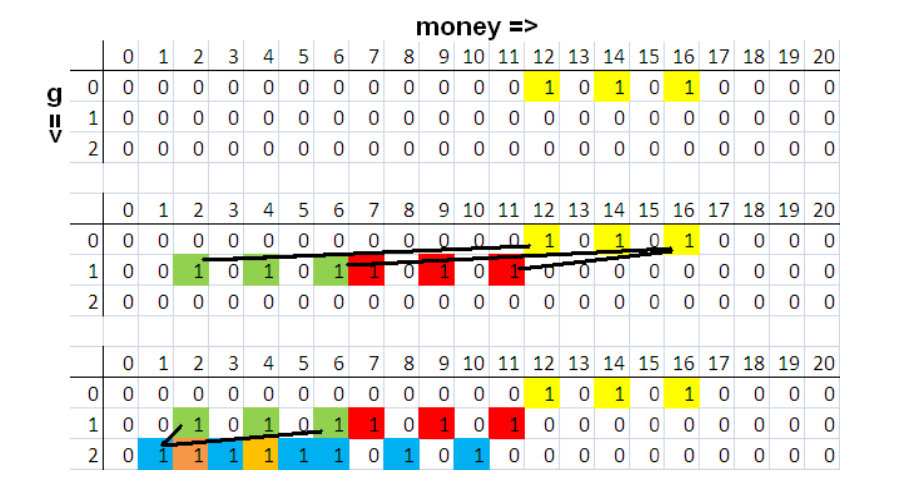
\includegraphics[scale=0.4]{imgs/11450_2.png}
    \caption{DP table when $g=1$ and $g=2$}
\end{figure}

\end{frame}

\begin{frame}[fragile]
\frametitle{UVa 11450: Bottom-Up DP Approach}

\begin{itemize}
    \item The answer can be found in the last row when \verb|g = C-1|
    \item Find the state in that row that is both nearest to index $0$ and reachable
    \item By looking at the DP table, we can see that the answer lies in \verb|reachable[2][1]|
    \item Meaning that we can reach state \verb|money = 1| by buying some combination of the various garment models
    \item \color{blue}The final answer is \verb|M - money = 20 - 1 = 19|\color{black}
    \item \color{red}\verb|C++ code: ch3_03_UVa11450_bu.cpp|\color{black}
\end{itemize}

\end{frame}

\begin{frame}[fragile]
\frametitle{Top-Down vs. Bottom-Up DP}

\begin{figure}
    \centering
    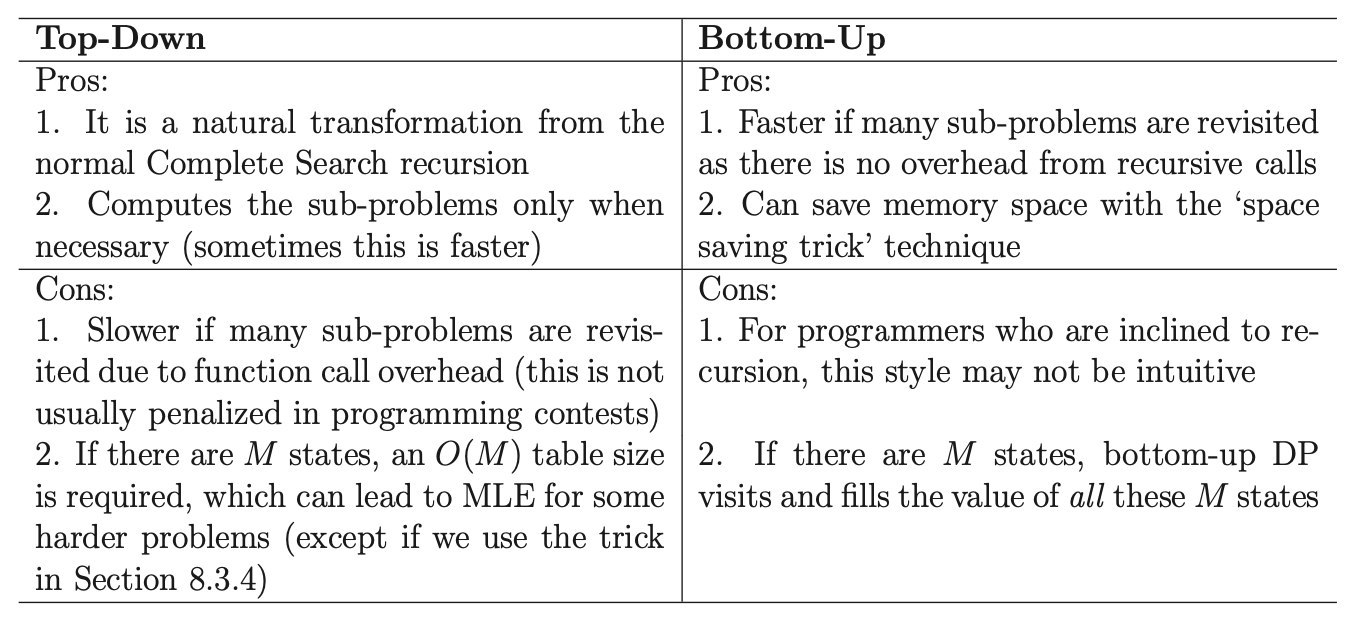
\includegraphics[scale=0.45]{imgs/td_vs_bu.png}
	\caption{Top-Down vs. Bottom-Up DP, \cite{Halim}:page 102}
\end{figure}

\end{frame}


%-------------------------------------------------------------------------------------
%-------------------------------------------------------------------------------------
%-------------------------------------------------------------------------------------
\subsection{2. Classical Problems}
\begin{frame}
	\frametitle{Table of Contents}
    \tableofcontents[currentsection, currentsubsection]	
\end{frame}

\begin{frame}[fragile]
\frametitle{DP Classical Problems}

\begin{itemize}
    \item \href{https://onlinejudge.org/index.php?option=com_onlinejudge&Itemid=8&category=26&page=show_problem&problem=2445}{UVa 11450} was an example of a non-classical DP problem
    \item However, there exists a list of classical DP problems (6) where the states and transitions are \textit{well-known}
    \item These problems should be mastered to perform well in ICPC in addition to its variants
\end{itemize}

\end{frame}

\begin{frame}[fragile]
\frametitle{DP Classical Problems}

\begin{enumerate}
    \item Max 1D Range Sum
    \item Max 2D Range Sum
    \item Longest Increasing Subsequence (LIS)
    \item 0-1 Knapsack (Subset Sum)
    \item Coin Change (CC) - General Version
    \item Traveling Salesman Problem (TSP)
\end{enumerate}

\end{frame}

%-------------------------------------------------------------------------------------
\begin{frame}[fragile]
\frametitle{1. Max 1D Range Sum}

\begin{itemize}
    \item \href{https://onlinejudge.org/index.php?option=com_onlinejudge&Itemid=8&category=7&page=show_problem&problem=448}{UVa 507 - Jill Rides Again}
    \item \color{red}\verb|C++ code: ch3_04_Max1DRangeSum.cpp|\color{black}
\end{itemize}

\vspace{0.3cm}

\color{red}\textbf{Problem Description: }\color{black} \\

Given an integer array $A$ containing $n \leq 20K$ non-zero integers, determine the maximum (1D) range sum of $A$. In other words, find the maximum Range Sum Query (RSQ) between two indices $i, j \in [0,\ldots,n-1]$, that is: $$A[i] + A[i+1] + A[i+2] +\ldots+ A[j]$$

\end{frame}

\begin{frame}[fragile]
\frametitle{1. Max 1D Range Sum}

\color{red}\textbf{DP strategy}\color{black} \\

\begin{itemize}
    \item Pre-process array \verb|A| by computing \verb|A[i]+=A[i-1]| $\forall i \in [1,\ldots,n-1]$ so that \verb|A[i]| contains the sum of integers in subarray \verb|A[0,...,i]|
    \item We can now compute \verb|RSQ(i,j)| in $O(1)$ as follows: \color{blue}\verb|RSQ(0,j)=A[j]| \color{black} and \color{blue}\verb|RSQ(i,j)=A[j]-A[i-1]| \color{black} $\forall i > 0$
\end{itemize}

\end{frame}

\begin{frame}[fragile]
\frametitle{1. Max 1D Range Sum}

\color{red}\textbf{Kadane's $O(n)$ Algorithm}\color{black} \\

\begin{itemize}
    \item Keeps a sum of the integers seen so far and greedily reset that to $0$ if the running sum dips below $0$
    \item Restarting from $0$ is better than continuing from a negative sum
    \item At each step we have two choices:
    	\begin{enumerate}
		    \item Keep using the accumulated maximum sum
		    \item Begin a new range
		\end{enumerate}
	\item \verb|ch3_04_Max1DRangeSum.cpp| uses the space saving trick
\end{itemize}


\end{frame}

%-------------------------------------------------------------------------------------
\begin{frame}[fragile]
\frametitle{2. Max 2D Range Sum}

\begin{itemize}
    \item \href{https://onlinejudge.org/index.php?option=com_onlinejudge&Itemid=8&category=3&page=show_problem&problem=44}{UVa 108 - Maximum Sum}
    \item \color{red}\verb|C++ code: ch3_05_UVa108.cpp|\color{black}
\end{itemize}

\vspace{0.3cm}

\color{red}\textbf{Problem Description}\color{black} \\

Given an $n \times n$ ($1 \leq n \le 100$) square matrix of integers $A$ where each integer ranges from $[-127,\ldots,127]$, find a sub-matrix of $A$ with the maximum sum. 

\end{frame}

\begin{frame}[fragile]
\frametitle{2. Max 2D Range Sum}

For example, the $4 \times 4$ matrix ($n = 4$) below has a $3 \times 2$ sub-matrix on the lower-left with maximum sum of $9 + 2 - 4 + 1 - 1 + 8 = 15$.

\begin{figure}
    \centering
    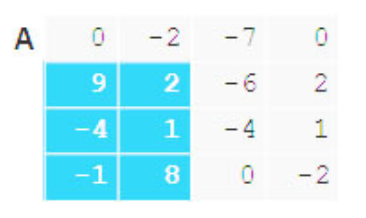
\includegraphics[scale=0.6]{imgs/max2d_1.png}
\end{figure}

\end{frame}

\begin{frame}[fragile]
\frametitle{2. Max 2D Range Sum}

\color{red}\textbf{DP strategy}\color{black} \\

\begin{itemize}
    \item The solution for the Max 1D Range Sum can be extended to two (or more) dimensions and we'll be dealing now with cumulative $n \times n$ sub-matrices
    \item \verb|A[i][j]| no longer contains its own value, but the sum of all items within sub-matrix $(0,0)$ to $(i,j)$
\end{itemize}

\end{frame}

\begin{frame}[fragile]
\frametitle{2. Max 2D Range Sum}

The code shown below turns the input square matrix into a cumulative sum matrix:

\vspace{0.3cm}

\begin{lstlisting}[language=c]
scanf("\%d", &n);
for (int i = 0; i < n; i++) for (int j = 0; j < n; j++) {
	scanf("\%d", &A[i][j]);
	if (i > 0) A[i][j] += A[i - 1][j];
	if (j > 0) A[i][j] += A[i][j - 1];
	if (i > 0 && j > 0) A[i][j] -= A[i - 1][j - 1];	
}\end{lstlisting}

\begin{figure}
    \centering
    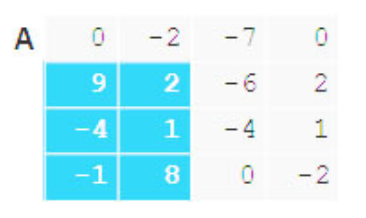
\includegraphics[scale=0.6]{imgs/max2d_1.png}
    \hspace{0.5cm}
    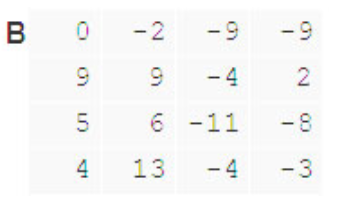
\includegraphics[scale=0.6]{imgs/max2d_2.png}
\end{figure}

\end{frame}

\begin{frame}[fragile]
\frametitle{2. Max 2D Range Sum}

To obtain the sum of a sub-matrix going from $(i,j)$ to $(k,l)$ in $O(1)$, we do the following:

\begin{itemize}
	\item \verb|sum = A[k][l]|
    \item If $i>0$, \verb|sum -= A[i-1][l]|
    \item If $j > 0$, \verb|sum -= A[k][j-1]|
    \item If $i>0$ and $j>0$, \verb|sum += A[i-1][j-1]|
\end{itemize}

\end{frame}

\begin{frame}[fragile]
\frametitle{2. Max 2D Range Sum}

For example, let’s compute the sum of $(1, 2)$ to $(3, 3)$:

\begin{itemize}
	\item \verb|sum = A[3][3] = -3|
    \item If $i>0$, \verb|sum -= A[0][3] = -9|
    \item If $j > 0$, \verb|sum -= A[3][1] = 13|
    \item If $i>0$ and $j>0$, \verb|sum += A[0][1] = -2|
    \item \color{blue}\verb|sum = -9|\color{black}
\end{itemize}

\begin{figure}
    \centering
    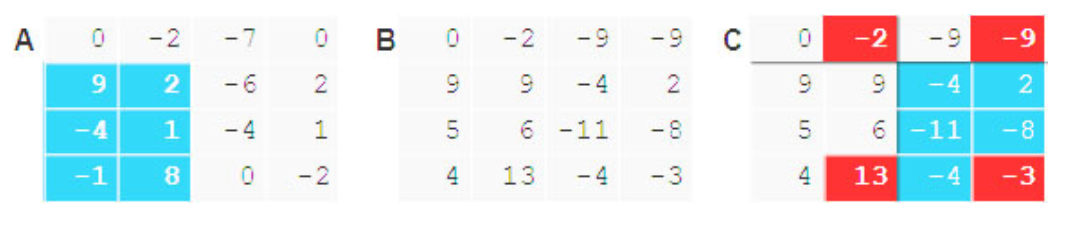
\includegraphics[scale=0.5]{imgs/max2d_3.png}
\end{figure}

\end{frame}


%-------------------------------------------------------------------------------------
\begin{frame}[fragile]
\frametitle{3. Longest Increasing Subsequence (LIS)}

\begin{itemize}
    \item \color{red}\verb|C++ code: ch3_06_LIS.cpp|\color{black}
\end{itemize} 

\vspace{0.3cm}

\color{red}\textbf{Problem Description: }\color{black} \\ 

Given a sequence $\{A[0], A[1],\ldots, A[n-1]\}$, determine its Longest Increasing Subsequence (LIS). Note that these \textit{subsequences} are not necessarily contiguous. 

\vspace{0.3cm}

For example, $n=8$, $A = \{-7,10,9,2,3,8,8,1\}$. The length-4 LIS is $\{-7, 2, 3, 8\}$

\end{frame}

\begin{frame}[fragile]
\frametitle{3. Longest Increasing Subsequence (LIS)}

\color{red}\textbf{Solution}\color{black} \\

\begin{itemize}
    \item Let \verb|LIS(i)| be the longest increasing subsequence ending at index \verb|i|
    \item Therefore, we can model this problem with one parameter: \verb|i|
    \pause
    \item \color{blue}\verb|LIS(0) = 1| \color{black} since the first number in \verb|A| is a subsequence
    \pause
    \item For \color{blue}\verb|LIS(i)| \color{black} given that $i \geq 1$ we need to do the following:
    
    	\begin{itemize}
			\pause
		    \item Find an index \verb|j| such that $j < i$
		    \pause
		    \item \verb|A[j] < A[i]|
		    
		    \pause
		    \item \verb|A[j]| must be the largest
		\end{itemize}
		
	\pause
	\item Once we found index \verb|j|, \color{blue}\verb|LIS(i) = LIS(j) + 1| \color{black}
    
\end{itemize}

\begin{figure}
    \centering
    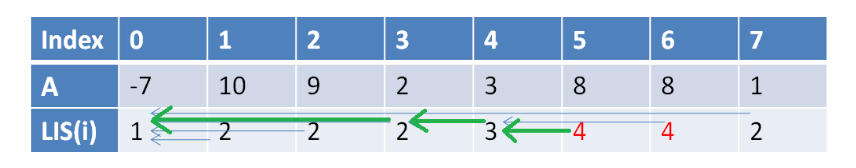
\includegraphics[scale=0.5]{imgs/lis_1.png}
\end{figure}

\end{frame}

\begin{frame}[fragile]
\frametitle{3. Longest Increasing Subsequence (LIS)}

We can write this recurrence formally as:

\begin{enumerate}
    \item \verb|LIS(0) = 1|, the base case
    \pause
    \item \verb|LIS(i) = max(LIS(j)+1)|, $\forall j \in [0,\ldots,i-1]$ and \verb|A[j] < A[i]|, the recursive case
\end{enumerate}

\vspace{0.3cm}

\pause
\color{blue}The answer is the largest value of \verb|LIS(k)| $\forall k \in [0,\ldots,n-1]$\color{black}

\begin{figure}
    \centering
    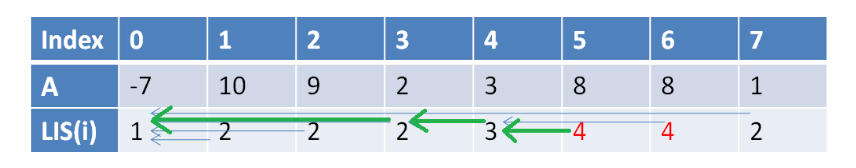
\includegraphics[scale=0.5]{imgs/lis_1.png}
\end{figure}

\end{frame}

\begin{frame}[fragile]
\frametitle{3. Longest Increasing Subsequence (LIS)}

\begin{itemize}
    \item Using the DP strategy described above, the algorithm will run in $O(n^2)$ time since we need to make a loop for each index $i$
    \item In addition to this, there are many overlapping sub-problems due to the same reason
    \item To further improve this algorithm, we could store the predecessor information and trace the green arrows from index \verb|k| that contains the largest value of \verb|LIS(k)|
\end{itemize}

\end{frame}

\begin{frame}[fragile]
\frametitle{3. Longest Increasing Subsequence (LIS)}

However, there is a solution using the Greedy and D\&C paradigms that runs in $O(n \log k)$:

\begin{itemize}
    \item Let array \verb|L| be an array such that \verb|L(i)| represents the smallest ending value of all length-$i$ LISs found so far
   	
	\pause
    \item \verb|L(i-i)| will always be smaller than \verb|L(i)|
    
   	\pause 
    \item Finally, we can binary search array \verb|L| to determine the longest possible subsequence we can create by appending the current element \verb|A[i]|
\end{itemize}

\end{frame}

%-------------------------------------------------------------------------------------
\begin{frame}[fragile]
\frametitle{4. 0-1 Knapsack (Subset Sum)}

\begin{itemize}
    \item \color{red}\verb|C++ code: ch3_07_UVa10130.cpp|\color{black}
\end{itemize} 

\vspace{0.3cm}

\color{red}\textbf{Problem Description: }\color{black} \\ 

Given $n$ items, each with its own value $V_i$ and weight $W_i$, $\forall i \in [0,\ldots,n-1]$, and a maximum knapsack size $S$, compute the maximum value of the items that we can carry, if we can either ignore or take a particular item (hence the term 0-1 for ignore/take)

\end{frame}

\begin{frame}[fragile]
\frametitle{4. 0-1 Knapsack (Subset Sum)}

For example, $n = 4$, $V = \{100,70,50,10\}$, $W = \{10,4,6,12\}$, $S = 12$.

\begin{itemize}
    \item If we select item 0 with weight 10 and value 100, we cannot take any other item. Not optimal
    \item If we select item 3 with weight 12 and value 10, we cannot take any other item. Not optimal
    \item If we select item 1 and 2, we have total weight 10 and total value 120. \textbf{This is the maximum}
\end{itemize}

\end{frame}

\begin{frame}[fragile]
\frametitle{4. 0-1 Knapsack (Subset Sum)}

Let's look at the following Complete Search recurrences for \verb|val(id, remW)| where \verb|id| is the index of the current item to be considered and \verb|remw| the remaining weight in the knapsack:

\begin{enumerate}
    \item \color{blue}\verb|val(id, 0) = 0|\color{black}, if \verb|remW = 0| we cannot take anything else
    \pause    
    \item \color{blue}\verb|val(n, remW) = 0 |\color{black}, if \verb|id = n| we have considered all items
    \pause
    \item \color{blue}\verb|if W[id] > remW|\color{black}, we have to ignore this item
    \begin{itemize}
        \item \verb|val(id, remW) = val(id + 1, remW)|
    \end{itemize}
    \pause
    \item \color{blue}\verb|if W[id] <= remW|\color{black}, we have two choices, either \color{orange}ignore \color{black} the item or \color{cyan}take \color{black} it. We take the one that gives us the maximum value:
\end{enumerate}


\hspace{0.6cm} \verb|val(id, remW) = | \\

\hspace{1cm} \verb|max(| \color{orange}\verb|val(id+1,remW), |\color{black} \color{cyan}\verb|V[id]+val(id+1,remW-W[id])|\color{black})


\end{frame}


%-------------------------------------------------------------------------------------
\begin{frame}[fragile]
\frametitle{5. Coin Change (CC) - General Version}

\begin{itemize}
    \item \color{red}\verb|C++ code: ch3_08_UVa674.cpp|\color{black}
\end{itemize} 

\vspace{0.3cm}

\color{red}\textbf{Problem Description: }\color{black} \\ 

Given a target amount $V$ cents and a list of denominations for $n$ coins, i.e. we have \verb|coinValue[i]| (in cents) for coin types $i \in [0,\ldots,n-1]$, what is the minimum number of coins that we must use to represent $V$ ? Assume that we have unlimited supply of coins of any type

\end{frame}

\begin{frame}[fragile]
\frametitle{5. Coin Change (CC) - General Version}

Let's look at the following Complete Search recurrences for \verb|change(value)| where \verb|value| is the remaining amount of cents that we need to represent in coins:

\begin{enumerate}
    \item \color{blue}\verb|change(0) = 0|\color{black}, we need 0 coins to produce 0 cents
    \pause
    \item \color{blue}\verb|change(< 0) = |$\infty$ \color{black}, we can return a large positive value
    
    \pause
    \item \color{blue}\verb|change(value) = 1+min(change(value-coinValue[i]))|\color{black}, $\forall i \in [0,\ldots,n-1]$    
\end{enumerate}

\begin{figure}
    \centering
    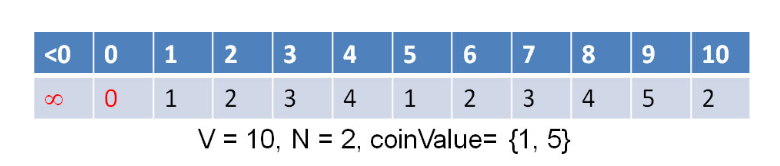
\includegraphics[scale=0.5]{imgs/cc.png}
\end{figure}

\end{frame}

\begin{frame}[fragile]
\frametitle{5. Coin Change (CC) - Alternative Version}

A variant of this problem is to count the number of possible (canonical) ways to get value V cents using a list of denominations of n coins. \\

\vspace{0.3cm}

For example, for $V=10$ above, the answer is $3: \{1+1+1+1+1 + 1+1+1+1+1, 5 + 1+1+1+1+1, 5 + 5\}$

\end{frame}

\begin{frame}[fragile]
\frametitle{5. Coin Change (CC) - Alternative Version}

Complete Search recurrences for \verb|ways(type, value)| where \verb|type| is the index of the coin type that we are currently considering:

\begin{enumerate}
    \item \color{blue}\verb|ways(type, 0) = 1|\color{black}, one way, just use nothing
    \item \color{blue}\verb|ways(type, <0) = 0|\color{black}, no way since we cannot reach a negative value    
    \item \color{blue}\verb|ways(n, value) = 0|\color{black}, no way since we have considered all coin types $\in [0,\ldots,n-1]$
    \item \color{blue}\verb|ways(type,value) = ways(type+1,value) + | \\ \verb|ways(type,value-coinValue[type])|\color{black}, if we ignore this coin type plus if we use this coin type
\end{enumerate}

\end{frame}


%-------------------------------------------------------------------------------------
\begin{frame}[fragile]
\frametitle{6. Traveling Salesman Problem (TSP)}

\begin{itemize}
    \item \href{https://onlinejudge.org/index.php?option=com_onlinejudge&Itemid=8&category=16&page=show_problem&problem=1437}{UVa 10496 - Collecting Beepers}
    \item \color{red}\verb|C++ code: ch3_09_UVa10496.cpp|\color{black}
\end{itemize} 

\vspace{0.3cm}

\color{red}\textbf{Problem Description: }\color{black} \\ 

Given $n$ cities and their pairwise distances in the form of a matrix \verb|dist| of size $n \times n$, compute the cost of making a tour that starts from any city $s$, goes through all the other $n-1$ cities exactly once, and finally returns to the starting city $s$.

\end{frame}

\begin{frame}[fragile]
\frametitle{6. Traveling Salesman Problem (TSP)}

For example, for $n=4$ cities, we have $4!=24$ possible tours (permutations of 4 cities). One of the minimum tours is \verb|A-B-C-D-A| with a cost of $20+30+12+35 = 97$

\begin{figure}
    \centering
    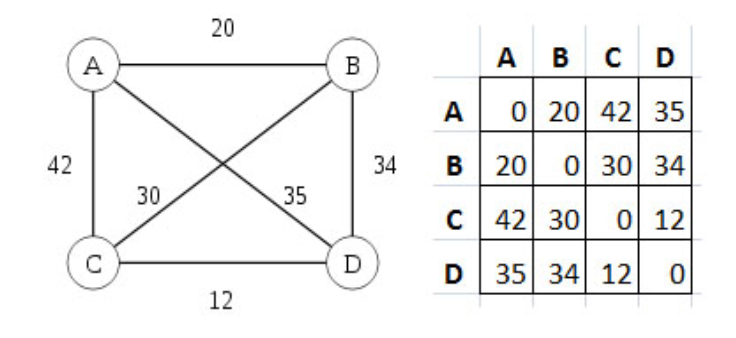
\includegraphics[scale=0.6]{imgs/tsp.png}
\end{figure}

\end{frame}

\begin{frame}[fragile]
\frametitle{6. Traveling Salesman Problem (TSP)}

\begin{itemize}
    \item TSP presents various overlapping sub-problems
    \begin{itemize}
        \item The tour \verb|A-B-C-(n-3)| other cities overlaps with the tour \verb|A-C-B-(n-3)| same other cities that also return to \verb|A|
    \end{itemize}
    \item If we can avoid re-computing various sub-tours we can save a lot of computation time
    \item Parameters for TSP: 
    \begin{enumerate}
        \item The last city visited: \verb|pos|
        \item Subset of the visited cities
    \end{enumerate}
\end{itemize}

\end{frame}

\begin{frame}[fragile]
\frametitle{6. Traveling Salesman Problem (TSP)}

\textbf{How do we represent a set?}

\vspace{0.3cm}

\begin{itemize}
    \item We need the set to be lightweight since it'll be used as a parameter in a recursive function
    \pause
    \item Solution: \textbf{bitmask}
    \item If we have $n$ cities, we could use an integer of length $n$
    \pause
    \item If the bit $i$ is $1$ (on), we say that the city with index $i$ has been visited (inside the set)
    \item Otherwise, it has not been visited yet ($i=0$, off)
\end{itemize}

\end{frame}

\begin{frame}[fragile]
\frametitle{6. Traveling Salesman Problem (TSP)}

\textbf{For example} 

\vspace{0.3cm}

\begin{itemize}
    \item \verb|mask| $ = 18_{10} = 10010_2$
    \item Implies that cities \textbf{1} and \textbf{4} have been visited
    \item To check if a bit $i$ is on or off: \verb|mask| $\& (1 << i)$
    \item To set bit $i$: \verb|mask| $|= (1 << i)$
\end{itemize}

\end{frame}

\begin{frame}[fragile]
\frametitle{6. Traveling Salesman Problem (TSP)}

Complete Search recurrences for \verb|tsp(pos, mask)|:

\begin{enumerate}
    \item \color{blue}\verb|tsp(pos,|$2^n$ \verb|-1) = dist[pos][0]|\color{black}, all cities have been visited
    \item \color{blue} \verb|tsp(pos, mask) = min(dist[pos][nxt] +| \\ \verb|tsp(nxt, mask| $|$ \verb|(1 << nxt)))|\color{black}, $\forall$ \verb|nxt| $\in [0,\ldots,n-1]$, \verb|nxt != pos| and \verb|(mask & (1 << nxt))| is $0$ (turned off). We try all possible next cities that have not been visited before at each step
\end{enumerate}

\end{frame}

\begin{frame}[fragile]
\frametitle{6. Traveling Salesman Problem (TSP)}

\begin{itemize}
    \item There are only $O(n \times 2^n)$ distinct states because there are $n$ cities and we remember up to $2^n$ other cities that have been visited in each tour
    \pause
    \item Each state can be computed in $O(n)$, thus the overall time complexity of this DP solution is$ O(2^n \times n^2)$
    
    \pause
    \item This allows us to solve up to $n \approx 16$ as $16^2 \times 2^{16} \approx 17M$
\end{itemize}

\pause
\vspace{0.3cm}

\color{blue}
This is not a huge improvement over the brute force solution but if the programming contest problem involving TSP has input size $11 \leq n \leq 16$, then DP is the solution, not brute force
\color{black}

\end{frame}


%-------------------------------------------------------------------------------------
%-------------------------------------------------------------------------------------
%-------------------------------------------------------------------------------------
\subsection{3. Non-Classical Problems}
\begin{frame}
	\frametitle{Table of Contents}
    \tableofcontents[currentsection, currentsubsection]	
\end{frame}

\begin{frame}[fragile]
\frametitle{DP Non-Classical Problems}

\begin{itemize}
    \item The classical DP problems in their pure forms usually never appear in modern ICPCs
    \item We'll discuss two more non-classical problems
    	\begin{enumerate}
		    \item \href{https://onlinejudge.org/index.php?option=com_onlinejudge&Itemid=8&category=21&page=show_problem&problem=1884}{UVa 10943 - How do you add?}
		    \item \href{https://onlinejudge.org/index.php?option=com_onlinejudge&Itemid=8&category=12&page=show_problem&problem=944}{UVa 10003 - Cutting Sticks}
		\end{enumerate}
\end{itemize}

\end{frame}


%-------------------------------------------------------------------------------------
\begin{frame}[fragile]
\frametitle{1. UVa 10943 - How do you add?}

\begin{itemize}
    \item \href{https://onlinejudge.org/index.php?option=com_onlinejudge&Itemid=8&category=21&page=show_problem&problem=1884}{UVa 10943 - How do you add?}
    \item \color{red}\verb|C++ code: ch3_10_UVa10943.cpp|\color{black}
\end{itemize}

\vspace{0.3cm}

\color{red}\textbf{Problem description}\color{black} \\

Given an integer $n$, how many ways can $K$ non-negative integers less than or equal to $n$ add up to $n$? Constraints: $1 \leq n, K \leq 100$

\pause
\vspace{0.3cm}

\textbf{For example}, for $n=20$ and $K=2$, there are $21$ ways: $0+20,1+19,2+18,3+17,\ldots,20+0$

\end{frame}


\begin{frame}[fragile]
\frametitle{1. UVa 10943 - How do you add?}

\begin{itemize}
    \item The number of ways can be expressed as $\begin{pmatrix} n+k-1 \\ k-1 \end{pmatrix}$ (Binomial Coefficient)
    \item However, we can solve this problem using DP techniques: parameters and transitions from one state to another given the base case or cases
\end{itemize}

\end{frame}

\begin{frame}[fragile]
\frametitle{1. UVa 10943 - How do you add?}


\begin{itemize}
    \item Parameters: tuple $(n,K)$
    \item \textbf{Base case}, when $K=1$, there is only one number less than or equal to $n$ to get $n$: $n$ itself
    \item \textbf{General case}, at state $(n,K)$ where $K>1$, we can split $n$ into $X \in [0,\ldots,n]$ and $n-X$, thus $n = X + (n-X)$
    \begin{itemize}
        \item By doing this, we arrive at the sub-problem $(n-X, K-1)$ which translates into \color{blue}"given a number $n-X$, how many ways can $K-1$ numbers less than or equal to $n-X$ add up to $n-X$?"\color{black}
        \item We can sum all these ways
    \end{itemize}
\end{itemize}

\end{frame}

\begin{frame}[fragile]
\frametitle{1. UVa 10943 - How do you add?}

Complete Search recurrences for \verb|ways(n,K)|:
\begin{enumerate}
    \item \verb|ways(n, 1) = 1|, since we can only use one number to add up to $n$, which is $n$ itself
    \item \verb|ways(n, k) = | $\sum_{X=0}^{n}$ \verb|ways(n - X, K - 1)|, sum all possible ways recursively
\end{enumerate}

\end{frame}


%-------------------------------------------------------------------------------------
\begin{frame}[fragile]
\frametitle{2. UVa 10003 - Cutting Sticks}

\begin{itemize}
    \item \href{https://onlinejudge.org/index.php?option=com_onlinejudge&Itemid=8&category=12&page=show_problem&problem=944}{UVa 10003 - Cutting Sticks}
    \item \color{red}\verb|C++ code: ch3_11_UVa10003.cpp|\color{black}
\end{itemize}

\vspace{0.3cm}

\color{red}\textbf{Problem description}\color{black} \\

Given a stick of length $1 \leq l \leq 1000$ and $1 \leq n \leq 50$ cuts to be made to the stick (the cut coordinates, lying in the range $[0,\ldots,l]$, are given). The cost of a cut is determined by the length of the stick to be cut. Your task is to find a cutting sequence so that the overall cost is minimized.


\end{frame}

\begin{frame}[fragile]
\frametitle{2. UVa 10003 - Cutting Sticks}

\textbf{For example}, $l=100$, $n=3$, and cut coordinates $A=\{25,50,75\}$

\vspace{0.3cm}

If we cut from left to right, we'll have a total cost of $225$:
\begin{enumerate}
    \item First cut is at coordinate $25$ (at original stick of length $l=100$), total cost so far $= 100$
    \item Second cut is at coordinate $50$ (at stick with length $75$), total cost so far $= 100 + 75 = 175$
    \item Third cut is at coordinate $75$ (at stick with length $50$), final total cost $= 175 + 50 = 225$
\end{enumerate}

\end{frame}

\begin{frame}[fragile]
\frametitle{2. UVa 10003 - Cutting Sticks}

However, the optimal answer is $200$:
\begin{enumerate}
    \item First cut is at coordinate $50$, total cost so far $= 100$
    \item Second cut is at coordinate $25$, total cost so far $= 100 + 50 = 150$
    \item Third cut is at coordinate $75$, final total cost $= 150 + 50 = 200$
\end{enumerate}

\begin{figure}
    \centering
    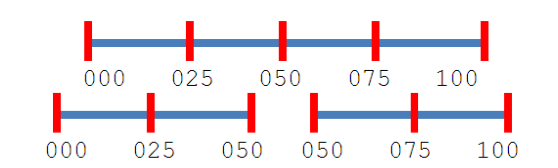
\includegraphics[scale=0.5]{imgs/cutting_sticks.png}
\end{figure}

\end{frame}

\begin{frame}[fragile]
\frametitle{2. UVa 10003 - Cutting Sticks}

\textbf{One possible solution}

\begin{itemize}
    \item Add two more coordinates to $A = \{0, \text{original A}, l\}$ so that we can denote later a stick by the indices of its endpoints in $A$
    
    \pause
    \item Define function \verb|cut(left, right)| that will return the cost of cutting at indices\footnote{left and right are the indices of the current stick with respect to A} \verb|left| and \verb|right|
    
    \pause
    \item Originally, the stick is described by \verb|left = 0| and \verb|right = |$n$\verb|+1|
\end{itemize}

\end{frame}

\begin{frame}[fragile]
\frametitle{2. UVa 10003 - Cutting Sticks}

\textbf{Complete Search recurrences}:

\begin{enumerate}
    \item \verb|cut(i-1, i) = 0|, $\forall i \in [1,\ldots,n+1]$, this stick segment does not need to be divided further since \verb|left + 1 = right|
    \item \verb|cut(left,right) = min(cut(left,i) + cut(i,right) +| \\ \verb|(A[right]-A[left]))|, $\forall i \in [$ \verb|left+1| $,\ldots,$ \verb|right-1| $]$, try all possible cutting points and pick the best (minimum)
\end{enumerate}

\vspace{0.3cm}
\color{blue}*The cost of a cut is the length of the current stick captured in \verb|(A[right]-A[left])|\color{black}

\end{frame}


%-------------------------------------------------------------------------------------
%-------------------------------------------------------------------------------------
%-------------------------------------------------------------------------------------
\subsection{4. DP in Programming Contests}
\begin{frame}
	\frametitle{Table of Contents}
    \tableofcontents[currentsection, currentsubsection]	
\end{frame}

\begin{frame}[fragile]
\frametitle{DP in Programming Contests}

Summary of the six classic DP problems:

\begin{figure}
    \centering
    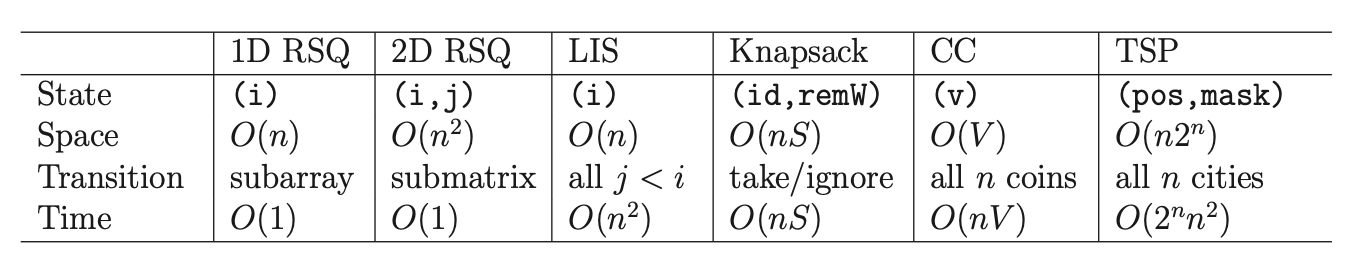
\includegraphics[scale=0.45]{imgs/classical_DP_problems.png}
\end{figure}

\end{frame}

\begin{frame}
\frametitle{DP in Programming Contests}

\begin{itemize}
    \item In addition to studying the non-classical examples, please check \href{https://www.topcoder.com/thrive/search?tags[]=Competitive\%20Programming\%20Tutorials}{Top Coder} for more DP tutorials 
    \item Mastering Dynamic Programming problems is now a basic requirement
    \item Art of DP: determining the states and knowing how to fill up the DP table (either TP or BU)
\end{itemize}

\end{frame}


%-------------------------------------------------------------------------------------
%-------------------------------------------------------------------------------------
%-------------------------------------------------------------------------------------
\subsection{5. Problems}
\begin{frame}
	\frametitle{Table of Contents}
    \tableofcontents[currentsection, currentsubsection]	
\end{frame}

\begin{frame}[fragile]
\frametitle{DP - Problems}

\begin{itemize}
    \item \href{https://onlinejudge.org/index.php?option=com_onlinejudge&Itemid=8&category=648}{UVa - DP problems}
    \item If UVa's site is not available, please check \cite{Halim}: page 115-117 for DP problems
    \item For problems' PDF's, please check \href{https://cpbook.net/methodstosolve?oj=both&topic=ch3&quality=all}{here}
\end{itemize}

\end{frame}

%-------------------------------------------------------------------------------------
%-------------------------------------------------------------------------------------
%-------------------------------------------------------------------------------------
\section*{References}
\begin{frame}{References}
    \begin{thebibliography}{}
        \bibitem[Halim]{Halim} Halim S., Halim F., \textit{Competitive Programming 3}, Handbook for ACM ICPC and IOI Contestants. 2013
        \bibitem[Skiean]{Skiena} Skiena S. \textit{The Algorithm Design Manual}. Springer. 2020
    \end{thebibliography}
\end{frame}

\end{document}
